\newpage


\section{Wstęp}\label{sec:wstep}

\subsection{Motywacja}\label{subsec:motywacja}

Sieć WWW (World Wide Web) w swoim pierwotnym założeniu została zaprojektowana z myślą o odczycie przez ludzi.
Od momentu powstania gwałtownie się rozrastała i tendencja ta wciąż się utrzymuje (zob. \autoref{fig:statista-data-volume-in-exabytes-per-month}).
Zważając na jej obecnie ogromny wolumen danych, ograniczone zasoby ludzkie pozwalają na przetworzenie jedynie niewielkiego ich ułamka.
W obliczu powyższych wyzwań niezbędna stała się więc technika web scrapingu polegająca na zbieraniu, ustrukturyzowaniu i przetworzeniu danych, tak aby umożliwić maszynom ich analizę.

\begin{figure}[H]
    \centering
    \captionsetup{width=.8\linewidth}
    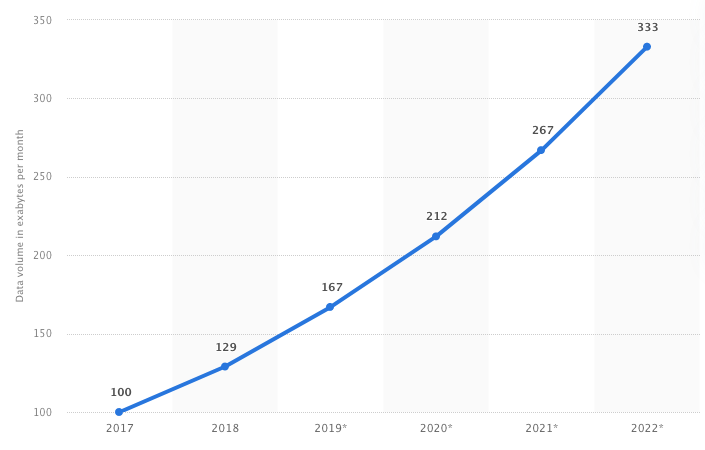
\includegraphics[width=\textwidth]{img/statista-data-volume-in-exabytes-per-month}
    \caption
        [Wolumen danych w globalnym konsumenckim ruchu IP w latach 2017–2022]
        {Wolumen danych w globalnym konsumenckim ruchu IP\\ w latach 2017–2022 (w eksabajtach na miesiąc)\\Źródło: \citetitle*{statista-data-volume}~\cite{statista-data-volume}}
    \label{fig:statista-data-volume-in-exabytes-per-month}
\end{figure}

Technika web scrapingu wciąż zyskuje na popularności stając się nieodzownym narzędziem w pracy z danymi.
Pozwala ona na szybkie i efektywne zbieranie ogromnych ilości danych.
Wykorzystuje się ją w wielu dziedzinach --- od badań społecznych, przez analizę konkurencji, po zbieranie danych do uczenia maszynowego i sztucznej inteligencji.
Skala zastosowania scraperów jest imponująca, co potwierdzają dane statystyczne.
W 2020 roku aż 37,2\% ruchu internetowego generowane było przez boty, w tym właśnie przez scrapery (zob. \autoref{fig:bot-traffic}).
Ta statystyka rzuca światło na ogromną rolę, jaką automaty internetowe odgrywają w cyfrowym ekosystemie.
Przy tak znacznej obecności botów, web scraping nie jest już tylko opcją, ale koniecznością dla tych, którzy chcą pozostać konkurencyjni w szybko rozwijającym się świecie danych.

\begin{figure}[H]
    \centering
    \captionsetup{width=.8\linewidth}
    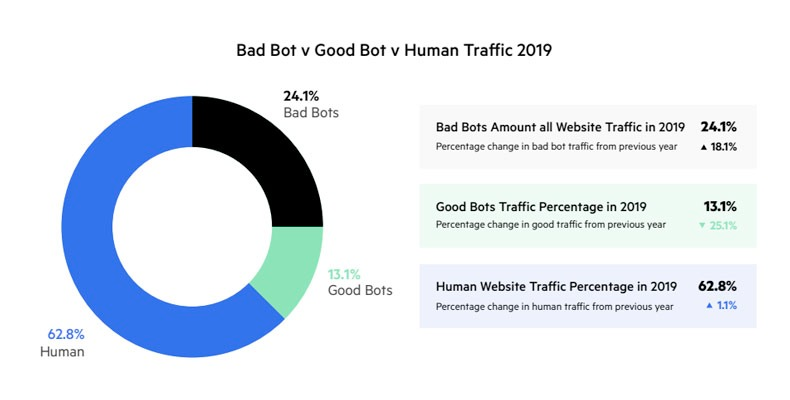
\includegraphics[width=\textwidth]{img/bot-traffic}
    \caption
        [Procentowy rozkład ruchu generowany w internecie przez: złe boty, dobre boty i ludzi w roku 2019]
        {Procentowy rozkład ruchu generowany w internecie przez:\\ złe boty, dobre boty i ludzi w roku 2019\\Źródło: \citetitle*{bot-traffic}~\cite{bot-traffic}}
    \label{fig:bot-traffic}
\end{figure}

Choć zastosowanie web scrapingu ma wiele zalet to wiąże się również z pewnymi zagrożeniami.
Firmy wykorzystują go do budowania przewagi konkurencyjnej, równocześnie dążąc do ochrony własnych danych przed podobnymi działaniami ze strony konkurencji.
W związku z tym, równolegle do rozwoju technik scrapingu rozwijane są metody jego detekcji i zapobiegania.

\subsection{Cel pracy}\label{subsec:cel-pracy}

Niniejsza praca posiada dwa główne cele.
Pierwszym jest analiza i praktyczne wykorzystanie web scrapingu.
Praca dąży do przedstawienia, zbudowania i przetestowania scrapera.
Drugim celem jest opracowanie i wdrożenie kilku różnych metod skutecznie blokujących web scraping.
Oba te cele mają pokazać zarówno perspektywę aktora przeprowadzającego scraping, jak i broniącego się przed nim.

\clearpage

\subsection{Struktura pracy}\label{subsec:struktura-pracy}

Praca ma charakter praktyczny i traktuje web scraping z dwóch perspektyw tj.~jego przeprowadzania oraz zabezpieczania się przed nim.
Składa się z 8 rozdziałów.
\begin{enumerate}[label={\textbf{Rozdział \arabic*}},labelindent=\parindent, leftmargin=*]
    \item \nameref{sec:teoria} stanowi teoretyczny wstęp do tematyki pracy.
    \item \nameref{sec:przeglad-rozwiazan} zawiera opis wybranych metod detekcji web scrapingu.
    \item \nameref{sec:projekt-platformy} koncentruje się na wdrożeniu sklepu internetowego tulski, który posłużył jako platforma do badań i testowania.
    \item \nameref{sec:projekt-scrapera} przedstawia proces projektowania i tworzenia scrapera pobierającego dane z sklepu tulski.
    \item \nameref{sec:wdrozenie-metod-detekcji} koncentruje się na praktycznym zastosowaniu metod detekcji web scrapingu, omawiając ich wdrożenie w kontekście stworzonego sklepu internetowego.
    \item \nameref{sec:wykorzystane-narzedzia} to prezentacja narzędzi i technologii wykorzystanych w pracy, w tym te służące do budowy sklepu, scrapera, jak również do wdrożenia zabezpieczeń.
    \item \nameref{sec:testy} przedstawia wyniki przeprowadzonych testów scrapera i sklepu wraz z zabezpieczeniami, a także dokonuje ich analizy.
    \item \nameref{sec:podsumowanie} podsumowuje główne tematy pracy, wnioski z badań i testów, a także zwraca uwagę na potencjalne kierunki dalszych badań w obszarze web scrapingu i jego detekcji.
\end{enumerate}
